\chapter{Conceptual solution}
\label{ch:concept}

This chapter introduces the proposed conceptual solution, which forms the basis for the implementation discussed in \cref{ch:impl}. Initially, an overview of the project structure is provided. Subsequently, the server-side infrastructure is examined, assessing the most suitable data model for use with \gls{a:mps} code generation, emphasizing key components, and ensuring thread-safe interactions among them. Finally, the client application is explored in depth, addressing its architecture, design, and quality of life enhancements.

\section{Project Infrastructure}

This section introduces the architectural solution designed to meet the requirements delineated in \cref{sec:requirements}. The comprehensive project architecture is illustrated in \cref{fig:architecture}, which encompasses three primary components: the client application, the server-side infrastructure, and the database.

\begin{figure}[H]
    \centering
    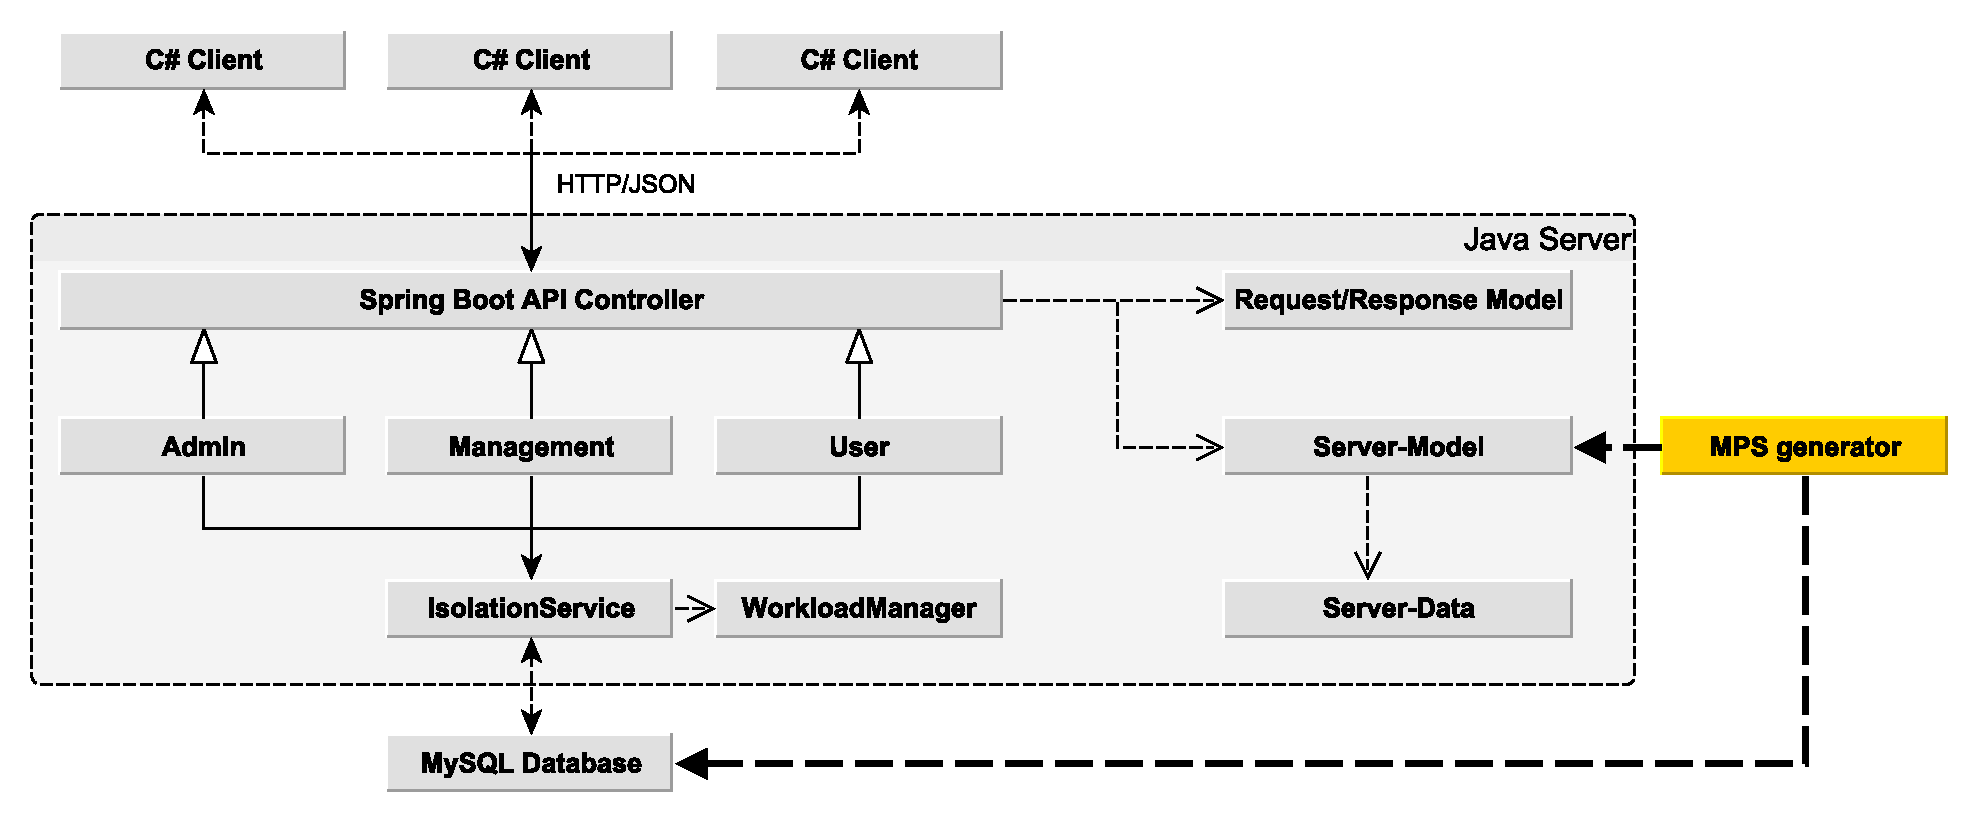
\includegraphics[width=\textwidth]{images/big-picture-no-lombok}
    \caption{Key aspects encompassing project architecture of the proposed solution.}
    \label{fig:architecture}
\end{figure}

\Cref{fig:architecture} illustrates the project architecture for the proposed solution. The architecture allows for multiple client application instances to connect concurrently to a single server instance, facilitating simultaneous user interactions. Communication between the client and server is achieved through a \gls{a:rest}ful \gls{a:json} \gls{a:api}, which adheres to standardized conventions and promotes interoperability between the C\# clients and the Java server. The design of the client is elaborated in further details in \cref{sec:cs-client}.

Upon invoking a specific endpoint using the client application, the server-side \gls{g:spring} \gls{a:api} controllers handle deserialization of the corresponding \gls{a:json} request model in accordance to the \gls{a:api} design specified in \cref{sec:cs-api}. These \gls{a:api} controllers subsequently process the request utilizing \gls{a:mps}-generated data access layer elucidated in \cref{sec:cs-data-model}, therefore ensuring a consistent, efficient, and maintainable interface with the underlying data storage.

The \inlinecode{IsolationService} plays a crucial role in managing and scheduling the data access requests performed by the \gls{a:api} controllers. It provides a level of isolation between concurrent requests, ensuring data consistency and preventing conflicts or race conditions. This service facilitates communication with the \gls{a:mps}-generated database schema, which is tailored to efficiently store and manage the system's data. A more comprehensive overview of the isolation service is provided in \cref{sec:cs-isolation}.

\section{Server}

The server application constitutes the central component of the \gls{g:cms}, overseeing the data model management and furnishing a \gls{a:rest} \gls{a:api} for client interactions. The implementation of the data model harnesses the \gls{a:mps} framework, while the \gls{a:rest} \gls{a:api} employs the \gls{g:spring} framework. Developed using Java, the server application capitalizes on the Maven build system. Ensuing sections provide a thorough analysis of the server application's architecture, commencing with an overview of the data model derived from the use-cases delineated in \cref{sec:use-cases}, continuing with an exposition of the \gls{a:rest} \gls{a:api}, and concluding with the presentation of the isolation layer.

\subsection{Data Model Design}\label{sec:cs-data-model}

The data model was created according to the requirements presented in chapter \ref{ch:problem-analysis}, see figure \ref{fig:data-model}. In order to provide a better orientation, the description of this figure should be from left to right.

\begin{figure}[H]
    \centering
    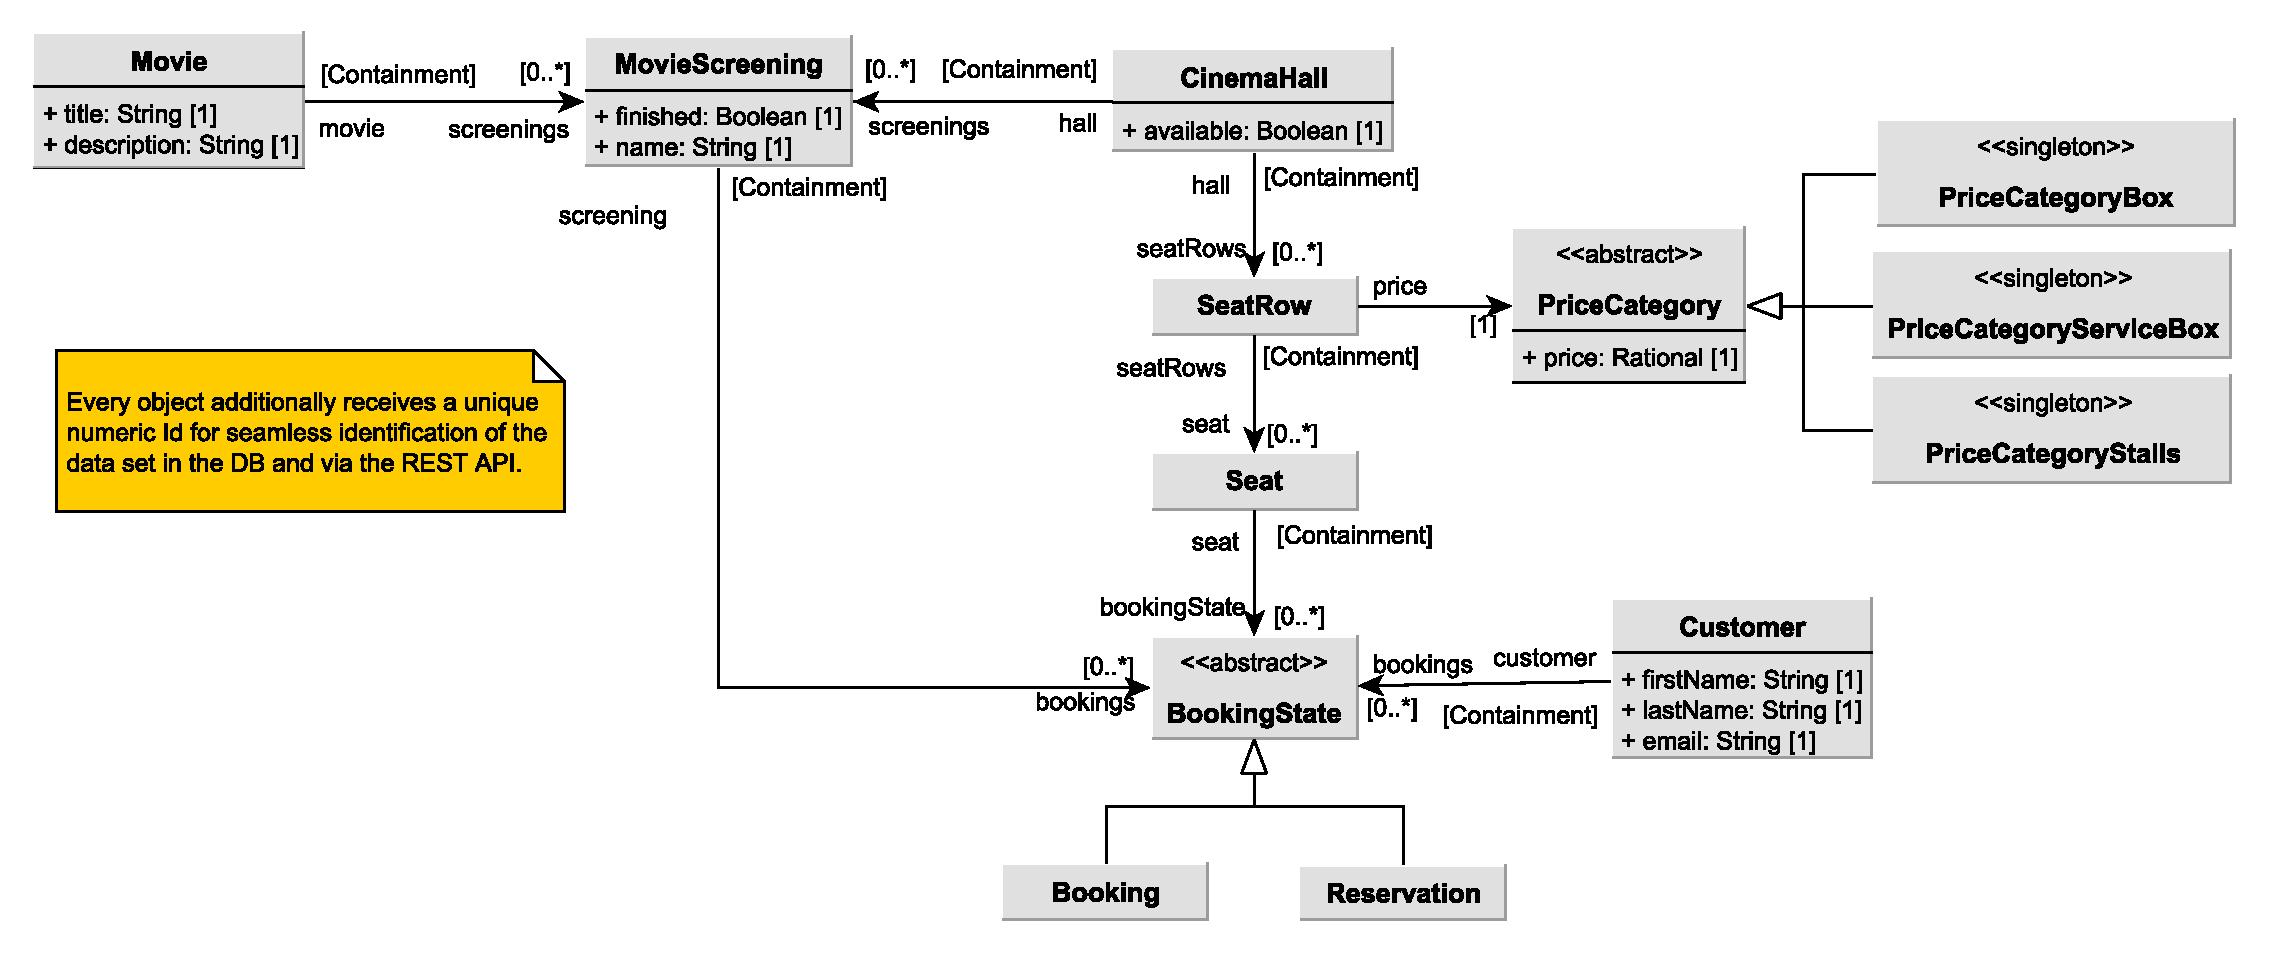
\includegraphics[width=\textwidth]{images/data-model-final-with-price}
    \caption{Data model for CMS according to requirements.}
    \label{fig:data-model}
\end{figure}

The class Movie contains two items, on the one hand a title as a string and on the other hand a description also as a string. The MoveScreening class contains two attributes according to the requirements. The attribute finished as a Boolean, indicates whether the film has finished screening and the attribute name as a string, identifies the name of each film screening. Between the classes Movie and MovieScreening there is an association as Containment. Furthermore, the CinemaHall class is required. It only has one attribute, namely whether the hall is currently in use. There is an association as containment within the CinemaHall and MovieScreening classes. Next, a class called SeatRow and another class Seat are necessary. The CinemaHall class and the SeatRow class have an association as a containment. There should also be a containment association from SeatRow to Seat. In addition, an abstract class BoookingState is needed for the booking system. This class is specified by the classes Reservation and Booking. There is again a containment association from the class to Seat to the abstract class BookingState. MovieScreening has a second association to BookingState, this one is also a containment. 
% you can use \inlinecode{MyClass} for code :)

\subsubsection{Compliance with MPS}

\todo{add subsubsections as needed!}

\todo{The UML diagram + formally proof containments for *all* relationships, e.g., A Seat Row cannot exist without a Cinama Hall and ...}

\todo{How do we need to change the model to comply with MPS? (Hint: enums and singletons)}

\pagebreak

\subsection{REST API}\label{sec:cs-api}

The \gls{a:rest} \gls{a:api} offers the client application an interface for interacting with the server. It comprises a set of \gls{a:rest}ful \gls{a:json} \gls{a:api} endpoints, with each endpoint handling a specific task.

\subsubsection{Endpoint Design}\label{sec:cs-api-endpoints}

To achieve a consistent and intuitive \gls{a:api} design, the endpoints were developed based on the use-cases outlined in \cref{sec:use-cases}. Consequently, the endpoints are initially grouped by the role responsible for performing the action, followed by the target of the action, and finally by the action itself. \Cref{fig:api-tree} illustrates a portion of the resulting tree structure of the \gls{a:api} endpoints, which is subsequently employed to create the Java \gls{g:spring} controllers.

\begin{figure}[H]
\renewcommand*\DTbaselineskip{10pt}
{\scriptsize
\dirtree{%
.1 \apiexpanded \ /.
.2 \apiexpanded management/. 
.3 \apicollapsed cinema-hall/ \apihandledby \syntaxcomplex{CinemaHallController}.
.3 \apiexpanded movie/ \apihandledby \syntaxcomplex{MovieController}.
.4 list \type \syntaxprimitive{GET} \apihandledby listMovies() \type \syntaxkeyword{GetMoviesResponse}.
.4 list-full \type \syntaxprimitive{GET} \apihandledby listDetailedMovies()\type \syntaxkeyword{GetMoviesFullResponse}.
.4 create \type \syntax[colorbrownish]{POST} \apihandledby createMovie(\syntaxkeyword{CreateMovieRequest})\type \syntaxkeyword{CreateMovieResponse}.
.4 update \type \syntax[colorbrownish]{POST} \apihandledby updateMovie(\syntaxkeyword{UpdateMovieRequest})\type \syntaxkeyword{UpdateMovieResponse}.
.4 delete \type \syntax[colorbrownish]{POST} \apihandledby deleteMovie(\syntaxkeyword{DeleteMovieRequest})\type \syntaxkeyword{DeleteMovieResponse}.
.3 \apicollapsed movie-screening/ \apihandledby \syntaxcomplex{MovieScreeningController}.
.3 \apicollapsed seat/ \apihandledby \syntaxcomplex{SeatController}.
.3 \apicollapsed seat-row/ \apihandledby \syntaxcomplex{SeatRowController}.
.2 \apiexpanded user/.
.3 \apicollapsed account/ \apihandledby \syntaxcomplex{UserAccountController}.
.3 \apicollapsed booking/ \apihandledby \syntaxcomplex{UserBookingController}.
.2 \apiexpanded admin/.
.3 \apicollapsed revenue/ \apihandledby \syntaxcomplex{AdminController}.
}
}
\renewcommand*\DTbaselineskip{20pt}
\raggedleft
{\scriptsize\vspace{-1cm}
\begin{tabular}{r@{ $\equalhat$ }l r@{ $\equalhat$ }l}
    \apicollapsed & \enquote{group collapsed} & \apiexpanded & \enquote{group expanded}\\
    \type & \enquote{is of type} & \apihandledby & \enquote{is handled by}\\
    \syntax[colorprimitive]{GET} & \enquote{\glsshort{a:http} GET request} & \syntax[colorbrownish]{POST} & \enquote{\glsshort{a:http} POST request}
\end{tabular}
\vspace{.25cm}}
\caption{Excerpt of the \gls{a:api} tree structure.}
\label{fig:api-tree}
\end{figure}

\Cref{fig:api-tree} presents an overview of all \gls{a:api} controllers and specifically of the endpoints within the \inlinecode{/management/movie} group. The \gls{a:api} endpoints are initially divided into three logical groups: \inlinecode{management}, \inlinecode{user}, and \inlinecode{admin}, each representing a different role. These logical groupings correspond to the Java packages containing the \gls{g:spring} controllers. On the second level, the endpoints are organized by their target, such as \inlinecode{movie} or \inlinecode{cinema-hall} for the management group. This second level maps to the respective Java \gls{g:spring} controller. Lastly, on the third level, endpoints are defined to handle the corresponding action, such as \inlinecode{list} or \inlinecode{create} for the movie controller. These endpoints map to the equivalent Java \gls{g:spring} controller methods.

Depending on the parameters necessary for executing the request action, either \inlinecode{GET} or \inlinecode{POST} requests are utilized. This is attributed to the fact that only \inlinecode{POST} requests can accommodate a body containing a \gls{a:json}-serialized request model. Consequently, communication through the \gls{a:api} is consistently \gls{a:json}-based. This approach simplifies the communication process, as both the client and server can effortlessly serialize and deserialize \gls{a:json} data, provided the \glspl{a:rrm} correspond. Additionally, \gls{a:json} is a prevalent choice for \gls{a:rest} \glspl{a:api} due to its lightweight nature, human readability, and compatibility with most programming languages, ensuring technology independence.

Java \gls{g:spring} controllers are tasked with converting \gls{a:json} request data into their respective Java request models and transforming Java response models into \gls{a:json} response data. To avert tight coupling and unintended cross-dependencies, each \gls{a:rrm} is exclusively employed by a single \gls{a:api} endpoint, facilitating model modification without the need for considering other endpoints. This encapsulation is illustrated in the simplified class diagram presented in \cref{fig:api-controllers}.

\begin{figure}[H]
\centering
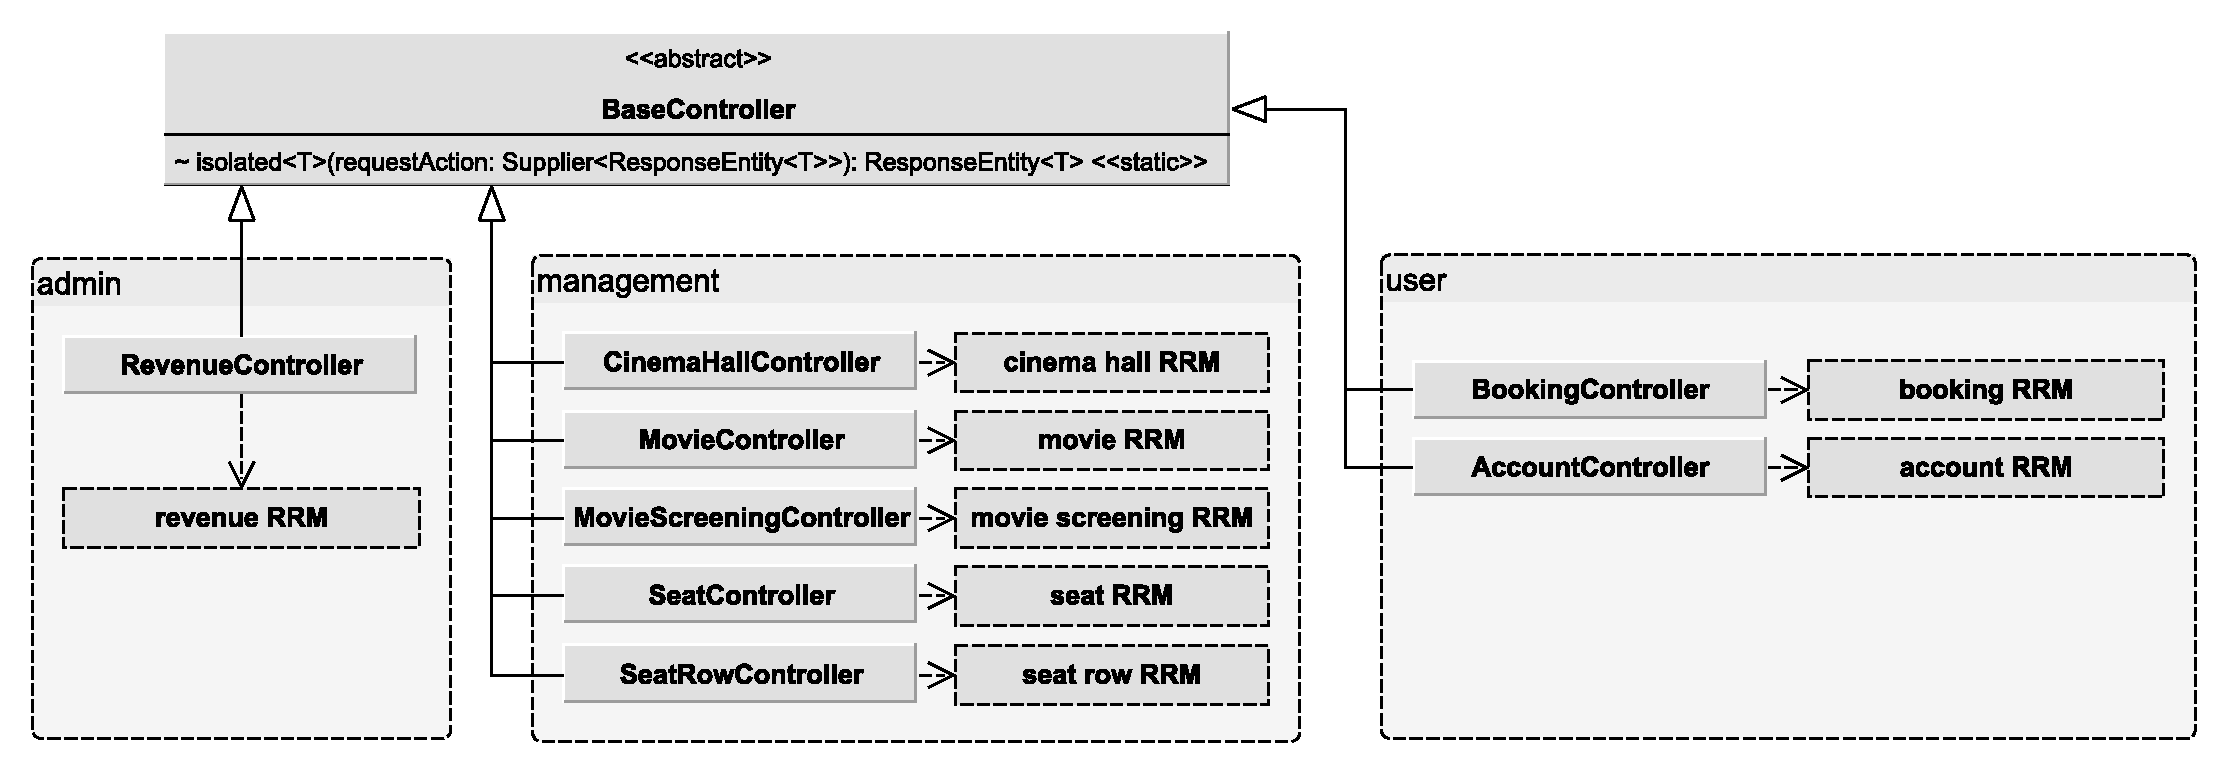
\includegraphics[width=\textwidth]{images/api-controllers}
\caption{Simplified \gls{a:api} controller structure with encapsulated \glspl{a:rrm}.}
\label{fig:api-controllers}
\end{figure}

However, the \gls{a:json}-based communication method presents a limitation, as it hinders the reusability of the existing \gls{a:mps} data model. This can be attributed to the fact that the generated classes can not easily be converted to \gls{a:json}, due to the reliance on the supervisor pattern. As a result, \glspl{a:rrm} are manually created and maintained separately. Future research could explore the potential for automatically generating \glspl{a:rrm} from the \gls{a:mps} data model. This approach would reduce manual maintenance efforts and enable the client to use the same data model as the server, thereby decreasing the likelihood of \gls{a:api} mismatches.

\subsubsection{API Controllers}\label{sec:cs-api-controllers}

The \gls{a:api} controllers, as depicted in \cref{fig:api-controllers}, are implemented as Java \gls{g:spring} controllers. Each controller is responsible for processing requests and producing responses, with every \gls{a:api} endpoint mapped to a single Java method within a controller.

To adhere to \cref{req:isolation}, a \inlinecode{BaseController} class is developed to streamline interactions with the isolation service, discussed in further detail in \vref{sec:cs-isolation}. This class offers the \inlinecode{isolated()} method, which simplifies the execution of a lambda function within the context of the isolation service. By carrying out the entire endpoint handling process within the isolation service, potential interleaving of database access by concurrent requests is avoided. Each \gls{a:api} controller extends the \inlinecode{BaseController} class, making the \inlinecode{isolated()} method accessible to all controllers. This approach reduces the complexity of the \gls{a:api} controllers, as the actual \gls{a:api} endpoint handling code does not need to address the isolation service directly. An illustrative example of employing the \inlinecode{BaseController} class is presented in \cref{lst:api-controllers-basecontroller}.

\begin{listing}[H]
\begin{minted}[fontsize=\scriptsize,linenos]{java}
@RestController
@RequestMapping(path="/api/foo", produces="application/json")
@CrossOrigin(origins="*")
public class FooController extends BaseController {
    @GetMapping("/bar")
    public ResponseEntity<BarResponse> getTheBar() {
        return isolated(() -> {
            // run business logic in isolated context...
            BarResponse response = ...
            return new ResponseEntity<BarResponse>(response, HttpStatus.OK);
        });
    }
}
\end{minted}
\caption{Utilization of the \inlinecode{isolated()} method in a concrete \gls{a:api} controller.}
\label{lst:api-controllers-basecontroller}
\end{listing}

\Cref{lst:api-controllers-basecontroller} demonstrates the use of the \inlinecode{isolated()} method within a concrete \gls{a:api} controller. As shown in line 7, the \inlinecode{isolated()} method accepts the request handling logic as a lambda function, which is executed in the context of the isolation service. The lambda function must return a \inlinecode{ResponseEntity} object containing the response data and the \gls{a:http} status code, which is then returned by the \inlinecode{isolated()} method. If an exception arises during the lambda function's execution, the isolation service automatically catches it and converts it into an error response with a suitable \gls{a:http} status code and stack trace information.

As illustrated in \cref{lst:api-controllers-basecontroller}, \gls{g:spring} mandates that the \inlinecode{ResponseEntity} be returned by the same controller method responsible for handling the request. This implies the execution within the isolation context to be, or appear to be, synchronous from an external perspective, as the controller method cannot return before the lambda function's execution is complete. This critical constraint must be taken into account when designing the isolation service, as asynchronous execution is not feasible. Consequently, this new requirement is formalized as \requirementdef\label{req:synchronous-isolation}.

\subsection{Isolation Service}\label{sec:cs-isolation}

As discussed in \cref{sec:cs-data-model}, the \gls{a:mps} framework is used to transform the data model into the required Java source code for the data access layer, concurrently generating a compatible database schema in MySQL to facilitate seamless database migrations. However, at the time of writing, the generated data access layer lacks isolation capabilities, rendering it incapable of handling transactional operations.

To enable concurrent data access from multiple clients, the server implements a custom isolation service atop the generated data access layer. This service is tasked with serializing concurrent accesses into a sequential chain of operations. Database operations are scheduled on a dispatch collection and executed by a self-balancing, bounded thread pool that supports various scheduling policies. The term \enquote{self-balancing} denotes that the quantity of worker threads varies depending on the load, while \enquote{bounded} refers to the ability to define an upper limit for concurrently active worker threads. A basic \gls{a:fifo} scheduling policy was selected for this application to prevent starvation and ensure fairness. Future enhancements could involve upgrading the basic \gls{a:fifo} queue to a priority heap structure, permitting more thorough control over scheduling, such as prioritizing management or administrative operations over user operations.

Although the thread pool theoretically maintains a flexible number of worker threads, adjusting dynamically based on the load, the maximum number of worker threads is practically limited to one to preserve the sequential execution of operations. Consequently, the thread pool effectively operates as a single-threaded queue. Nevertheless, the overall design could accommodate parallel execution of database operations in the future if the data model were expanded to support it.

To ensure compatibility with the \gls{g:spring} \gls{a:api} controllers, the isolation service must operate synchronously, as \gls{g:spring} anticipates that the thread handling a request will also be accountable for sending the response back to the client. This compatibility concern was identified in \cref{sec:cs-api} and subsequently incorporated as \cref{req:synchronous-isolation} for the isolation layer.

\pagebreak

\subsubsection{Workload Management}

As depicted in \cref{fig:workload-overview}, the isolation service (\inlinecode{IsolationService}) serves as an entry-point  for the highly configurable \inlinecode{WorkloadManager} class. While the \inlinecode{WorkloadManager} is responsible for maintaining the dispatch queue and worker thread pool, the \inlinecode{IsolationService} merely introduces an additional layer of abstraction, serving as a facade to encapsulate the intricacies of workload management. As such, a singular \inlinecode{schedule()} method is exposed, mapping a provided lambda expression to a workload object, which the caller can use to block until the operation is completed and to retrieve the results. This approach facilitates seamless integration with the \gls{g:spring} \gls{a:api} controllers, as no callbacks are necessary. The following paragraphs aim to offer a more comprehensive description of this execution process.

\begin{figure}[H]
\centering
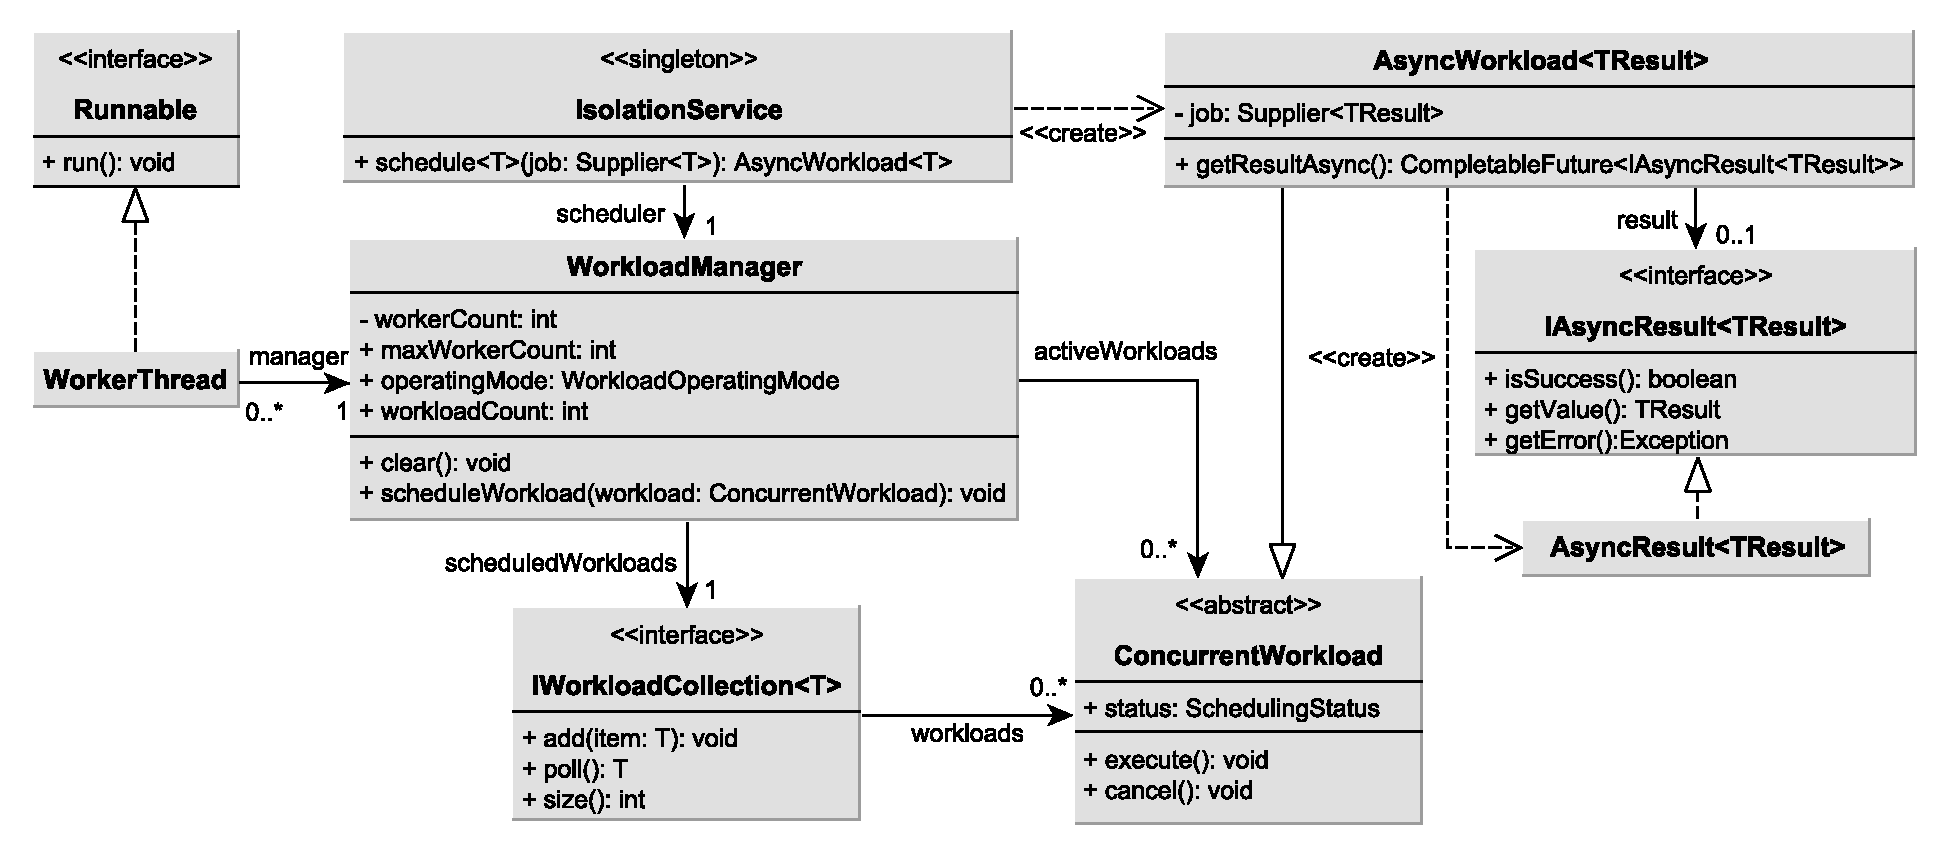
\includegraphics[width=\textwidth]{images/workload-management.pdf}
\caption{Simplified class diagram of the isolation service}
\label{fig:workload-overview}
\end{figure}

When scheduling an operation of type \inlinecode{Supplier<TResult>}, the \inlinecode{IsolationService} instantiates a new \inlinecode{AsyncWorkload<TResult>} object, which is then placed onto the dispatch queue. Subsequently, it returns the workload object to the caller, who can then obtain the \inlinecode{CompletableFuture<IAsyncResult<TResult>>} object from the workload object and utilize it to block until the operation is completed and to retrieve the results.

Simultaneously, scheduling the workload induces the \inlinecode{WorkloadManager} to attempt to adjust the number of active workers. Initially, a synchronization lock is acquired to guarantee that the active worker count remains consistent while subsequent steps are performed. The \inlinecode{WorkloadManager} then checks if the maximum worker count has been reached; if not, the number of active workers is incremented by one, and a new worker thread is created. The caller releases the synchronization context and the new worker thread tries to dequeue workloads from the dispatch queue for execution. This process begins by acquiring another synchronization lock specific to the dispatch queue. Following this, another check is initiated to verify and adjust the worker counts, assuring that the new worker thread is still required and that the number of allowed threads was not altered since the last check.

If the upper boundary of threads has been violated, the worker thread terminates and another existing thread handles execution of the scheduled workload. Otherwise if the upper limit has not yet been reached and more workloads are available, an additional worker thread is created. In any case other than termination, the worker thread attempts to dequeue a workload from the dispatch queue. If the dispatch queue is empty, the thread decrements the active worker count by one, and terminates. Otherwise, the worker thread assesses whether the workload was canceled while waiting in the dispatch queue; if so, it retrieves the next workload from the queue. In any other ways, the workload is set to \inlinecode{SchedulingStatus.Executing}, forestalling attempts to cancel it, and the worker thread carries on with workload execution, invoking the provided lambda expression and storing the result by completing the corresponding \inlinecode{Future}  object in the \inlinecode{AsyncWorkload}. If an exception is raised in client code during execution, the Future is completed with the exception object. Finally, this process is repeated until the dispatch queue is empty, and the number of active workers is reduced to zero.

Once the \inlinecode{Future} object is completed, the calling \gls{a:api} controller thread unblocks, and a response is transmitted back to the client.

\pagebreak

\section{Client}
\label{sec:cs-client}

This section presents the client application, which is the interface through which the user interacts with the system. The client application conforms to \cref{req:client-portability} (portability) by utilizing the most recent C\# 11/.NET 7 \gls{a:sdk}. C\# was chosen over Java, primarily due to a reduction of boilerplate code and greater portability, as the application can be published with a self-contained trimmed \gls{a:cclr}, eliminating the dependency on a separate .NET runtime installation. Additionally, the authors are more familiar with C\#, making it a natural choice.

\subsection{Introduction}

Despite being designed as a command line interface without a graphical user interface, it strives to maintain an intuitive and user-friendly experience, enabling users to efficiently manage the cinema system on a day-to-day basis. Cinema employees utilize the application for creating, modifying, and deleting movies, cinema halls, seat rows, seats, and showtimes, while customers use it for booking and canceling tickets. Additionally, the client application supports administrative tasks, such as analyzing movie and showtime revenue. Consequently, the client application must differentiate between three use-case sets: \inlinecode{management}, \inlinecode{user}, and \inlinecode{administration} (abbreviated as \inlinecode{admin}).

To prioritize accessibility, commands are designed for intuitive and natural interaction. The first command layer corresponds to use-case groups, while the second layer denotes specific operations (\gls{a:crud}). Common aliases are provided for each command, allowing users to select their preferred syntax. Each command specifies a target for the operation, resulting in a three-part structure: the use-case group, specific operation, and target. For instance, \inlinecode{management create movie} and \inlinecode{user create booking} are valid commands. A \inlinecode{help} command facilitates \gls{a:cli} navigation, displaying available commands and options depending on the user's position within the command tree. For example, \inlinecode{management help} lists all available management commands, while \inlinecode{management create help} enumerates valid targets for the create command in the management context.

The subsequent sections delve into the components required for implementing these features. \Cref{sec:cs-cli} examines the \gls{a:cli} parser, \cref{sec:cs-api-access} discusses the infrastructure necessary for server access, and \cref{sec:cs-autocomplete} introduces the autocomplete layer.

\subsection{Command line parsing}\label{sec:cs-cli}

%System.CommandLine framework and command processing

A primary concern for the client involves developing an intuitive command line interface. To tackle this issue, the \inlinecode{System.CommandLine} framework is employed for parsing \gls{a:cli} commands and arguments. Consequently, a hierarchical command-argument structure is established to facilitate the interpretation of user input. The syntax tree depicted in \cref{fig:command-tree} illustrates the command structure available to the client. It is essential to note that the root node functions solely as a logical container for the main commands.
\begin{minipage}[t]{0.45\textwidth}
The child nodes of the root node comprise management, user, and admin commands, which align with the distinct use-case groups identified in \cref{sec:use-cases}. Management sub-commands are generalized into the \inlinecode{ManagementCommand} class, which defines common management target arguments, represented as enums, employed by the concrete \gls{a:crud} commands that extend the \inlinecode{ManagementCommand} class.

The user sub-tree is similarly divided into create, read, update, and delete commands. However, these sub-commands are not consolidated into a single class, as they may not share identical arguments. For example, customers can create ticket reservations and bookings, but only ticket reservations may be cancelled. An optional \inlinecode{--as-identity} option may be utilized to specify the user or customer identity for performing the designated action. If no identity is specified, the user% don't touch this lol
\end{minipage}
\hfill
\begin{minipage}[t]{0.6\textwidth}
\vspace{-.5cm}
\begin{figure}[H]
\renewcommand*\DTbaselineskip{10pt}
{\scriptsize
\dirtree{%
.1 root \type \syntaxcomplex{RootCommand}.
.2 management \extends \syntaxcomplex{Command}.
.3 \syntaxcomplex{ManagementCommand} \syntaxkeyword{<<abstract>>} \extends \syntaxcomplex{Command}.
.4 movies \type \syntaxprimitive{ManagementOperationTarget}.
.4 screenings \type \syntaxprimitive{ManagementOperationTarget}.
.4 halls \type \syntaxprimitive{ManagementOperationTarget}.
.4 rows \type \syntaxprimitive{ManagementOperationTarget}.
.4 seats \type \syntaxprimitive{ManagementOperationTarget}.
.3 create \extends \syntaxcomplex{ManagementCommand}.
.3 read \extends \syntaxcomplex{ManagementCommand}.
.3 update \extends \syntaxcomplex{ManagementCommand}.
.3 delete \extends \syntaxcomplex{ManagementCommand}.
.2 user \extends \syntaxcomplex{Command}.
.3 {-}-as-identity \type \syntaxcomplex{Option}.
.4 identity \type \syntaxprimitive{string}.
.3 create \extends \syntaxcomplex{Command}.
.4 user \type \syntaxprimitive{UserCreateCommandTarget}.
.4 booking \type \syntaxprimitive{UserCreateCommandTarget}.
.4 reservation \type \syntaxprimitive{UserCreateCommandTarget}.
.3 read \extends \syntaxcomplex{Command}.
.4 users \type \syntaxprimitive{UserReadCommandTarget}.
.4 bookings \type \syntaxprimitive{UserReadCommandTarget}.
.4 reservations \type \syntaxprimitive{UserReadCommandTarget}.
.3 update \extends \syntaxcomplex{Command}.
.4 reservation \type \syntaxprimitive{UserUpdateCommandTarget}.
.3 delete \extends \syntaxcomplex{Command}.
.4 user \type \syntaxprimitive{UserDeleteCommandTarget}.
.4 reservation \type \syntaxprimitive{UserDeleteCommandTarget}.
.3 book \syntaxkeyword{<<alias>>} \extends \syntaxcomplex{Command} $\implies$ create booking.
.3 reserve \syntaxkeyword{<<alias>>} \extends \syntaxcomplex{Command} $\implies$ create reservation.
.3 cancel \syntaxkeyword{<<alias>>} \extends \syntaxcomplex{Command} $\implies$ delete reservation.
.2 admin \extends \syntaxcomplex{Command}.
.3 show \extends \syntaxcomplex{Command}.
.4 revenue \type \syntaxprimitive{AdminReadCommandTarget}.
}
}
\renewcommand*\DTbaselineskip{20pt}
\caption{The client command syntax tree.}
\label{fig:command-tree}
\end{figure}
\end{minipage}
\vspace{-.25cm}

will be prompted to enter their respective email address in a subsequent step. Finally, a collection of alias commands are incorporated into the user command, which directly correspond to their respective \gls{a:crud} commands.

The admin sub-tree shares similarities with the user sub-tree but consists solely of the read command, employed to display the revenue of a specified movie or movie screening.

\subsubsection{Class Design}

To implement \gls{a:cli} commands in a structured and maintainable fashion, the \inlinecode{System.CommandLine} framework is encapsulated within a class hierarchy, as illustrated in \vref{fig:command-classes}.

\begin{figure}[H]
    \centering
    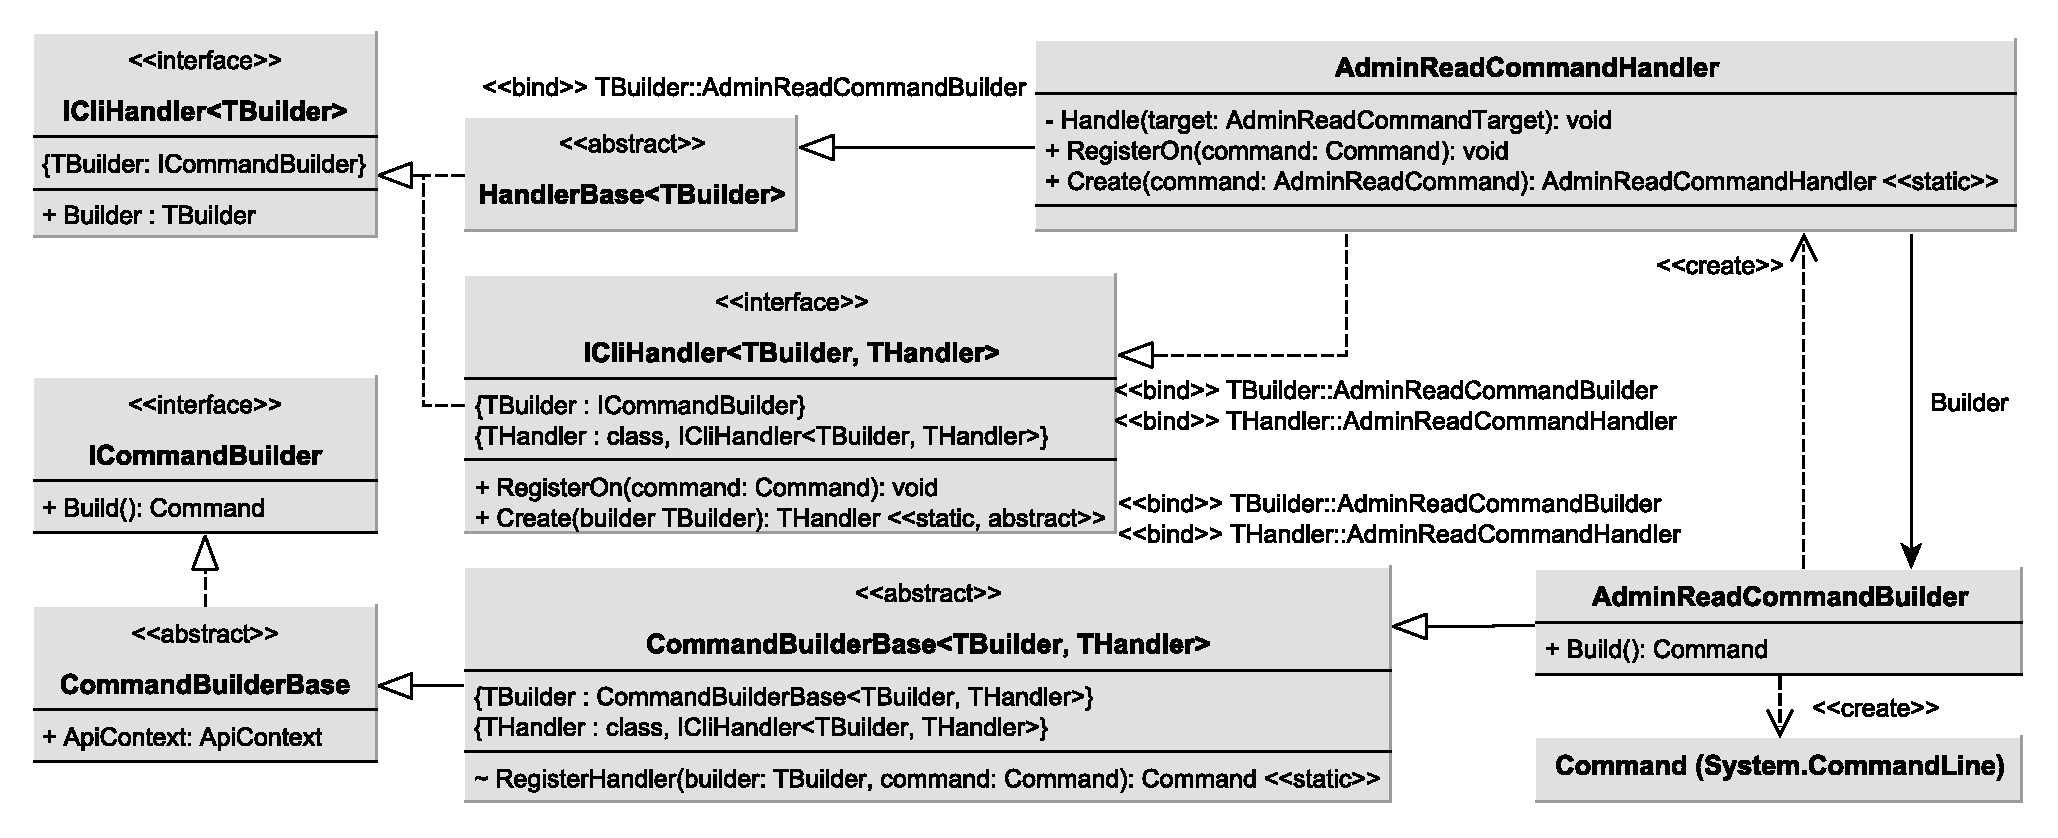
\includegraphics[width=\textwidth]{images/client-cli-command-parsing.pdf}
    \caption{Class hierarchy of the \gls{a:cli} command parsing framework.}
    \label{fig:command-classes}
\end{figure}

\Cref{fig:command-classes} displays the fundamental classes and interfaces of the command tree, along with an exemplary implementation of the \inlinecode{admin show} command.

The class hierarchy can be divided into command builders and command handler classes. Command builders serve to define and configure \inlinecode{System.CommandLine} command objects and their respective arguments. Command handler classes are responsible for configuring sub-commands on the \inlinecode{System.CommandLine} command objects within their corresponding \inlinecode{RegisterOn} methods and managing command execution through their \inlinecode{Handle} methods.

The configuration workflow generally adheres to the following steps:

\begin{enumerate}
    \item A command builder is instantiated and configured with the required arguments.
    \item The \inlinecode{builder.Build()} method is called to create and configure the \inlinecode{System.CommandLine} command object.
    \item The command object is added to the parent or root command object.
    \item The newly created command object is passed to the \inlinecode{RegisterHandler} method in the abstract \inlinecode{CommandBuilderBase} class, which subsequently generates the respective command handler using the static abstract \inlinecode{Create} factory method on the \inlinecode{THandler} type parameter.
    \item The \inlinecode{RegisterHandler} method calls the \inlinecode{RegisterOn} method on the command handler instance, which is accountable for registering sub-commands on the \inlinecode{System.CommandLine} command object. This is accomplished by instantiating one or more new command builders and passing them an instance of their corresponding parent, restarting from step 1.
\end{enumerate}

Consequently, each node in the syntax tree presented in \cref{fig:command-tree} is represented by an implementation of the \inlinecode{ICommandBuilder} interface, which in turn possesses a corresponding handler to recursively configure child command builder nodes. This arrangement offers a coherent and maintainable structure for the command tree, which can be effortlessly extended by incorporating new command builders and handlers for additional commands and their respective sub-commands.

A challenge presented by this command tree design involves the necessity to propagate global options, such as the \inlinecode{--as-identity} option in the user command sub-tree, from parent nodes to their child nodes. This is essential since the sole approach of obtaining the values of global options in the Handle methods of leaf nodes is via the original \inlinecode{System.CommandLine} option instance, configured by the parent command builder. As a result, any such options are stored within the respective command builder, which can then be injected into the corresponding command handler and passed down to subsequent layers of the command tree. To facilitate this process, C\# 11's support for static abstract interface members is employed. This enables the \inlinecode{Create} factory method to be defined and invoked using the associated generic type parameter \inlinecode{THandler}, mitigating the need for a separate factory object, or for explicit casts on the callee side if a generic factory is used. This design pattern is demonstrated in \cref{lst:command-builder-static-abstract-interface-members}.

\begin{listing}[H]
\begin{minted}[fontsize=\scriptsize,linenos,mathescape]{csharp}
public interface ICliHandler<TBuilder, THandler> : ICliHandler<TBuilder>
    where TBuilder : ICommandBuilder 
    where THandler : class, ICliHandler<TBuilder, THandler> 
{
    ...
    static abstract THandler Create(TBuilder builder); // static abstract factory method$\label{lst:ln:THandler-definition}$
}

public abstract class CommandBuilderBase<TBuilder, THandler> : CommandBuilderBase
    where TBuilder : CommandBuilderBase<TBuilder, THandler>
    where THandler : class, ICliHandler<TBuilder, THandler>
{
    ...
    // the generic RegisterHandler implementation
    protected static Command RegisterHandler(TBuilder builder, Command command)
    {
        // invocation of static method on the THandler type parameter which is known to 
        // implement the corresponding ICliHandler interface
        THandler handler = THandler.Create(builder); // use static interface method$\label{lst:ln:THandler-usage}$
        handler.RegisterOn(command);
        return command;
    }
}
\end{minted}
\caption{Utilization of a static abstract factory interface in the generic \inlinecode{RegisterHandler} implementation.}
\label{lst:command-builder-static-abstract-interface-members}
\end{listing}

\Vref{lst:command-builder-static-abstract-interface-members} presents the definition of the static abstract factory method in \inlinecode{ICliHandler} in \lref{lst:ln:THandler-definition} and its usage in the generic implementation of the \inlinecode{RegisterHandler} method in \lref{lst:ln:THandler-usage}. Generic constraints on the type parameters of \inlinecode{CommandBuilderBase} and \inlinecode{ICliHandler} ensure the appropriate command handler is created and registered for the corresponding command builder, eliminating the need for explicit casts or type checking.

\subsection{API Access}\label{sec:cs-api-access}

Upon command execution, the corresponding command handler class assumes responsibility for managing the command's execution.

Since the majority of leaf nodes in the command tree correspond to enums, the respective enum value is passed to the command handler, which subsequently switches on its value and invokes the appropriate \inlinecode{RemoteOperation} delegate. The \inlinecode{RemoteOperation} delegate refers to a method in the associated \inlinecode{Operation} class, which is specific to the handler and is accountable for performing one or more \gls{a:api} calls relevant to the requested operation. This approach enables command handler classes to remain independent of the actual \gls{a:api} calls, concentrating solely on managing the command's execution and promoting a cleaner separation of concerns. The hierarchy of user operation classes depicted in \cref{fig:client-operations} serves as a representative example for other operation class hierarchies.

\begin{figure}[H]
    \centering
    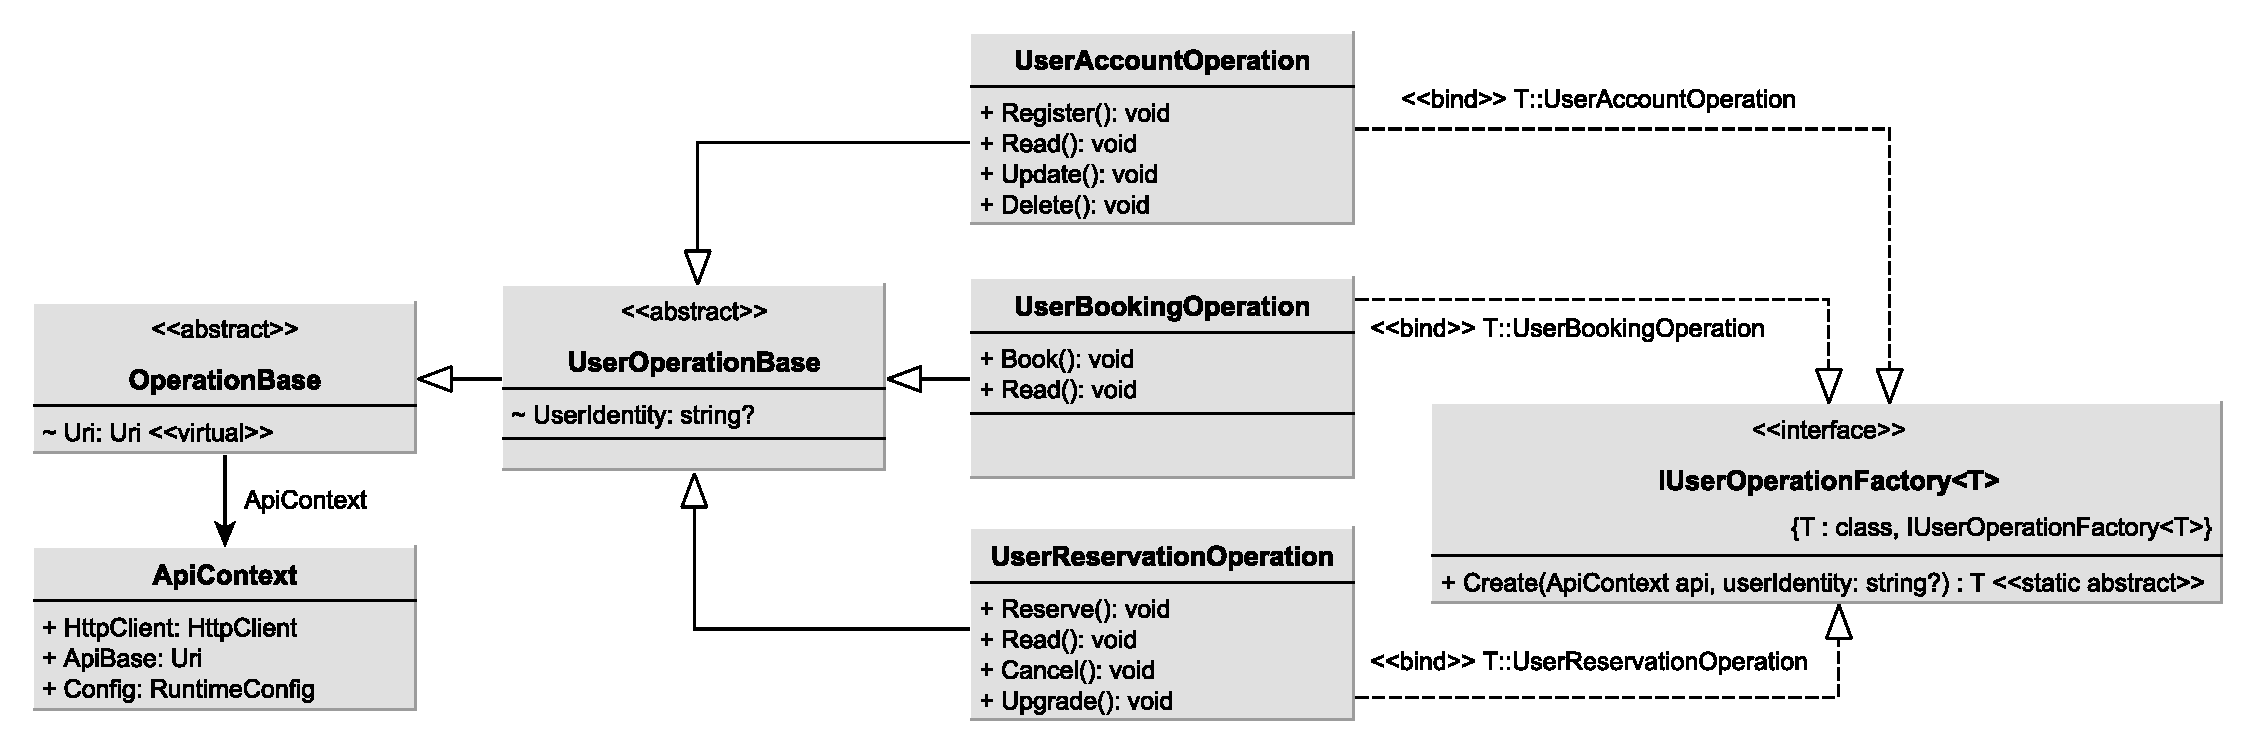
\includegraphics[width=\textwidth]{images/client-operations}
    \caption{User operation class hierarchy.}
    \label{fig:client-operations}
\end{figure}


As illustrated in \cref{fig:client-operations} the \inlinecode{OperationBase} class maintains a reference to an \inlinecode{ApiContext} object, responsible for storing the \inlinecode{HttpClient} instance utilized for all \gls{a:api} calls, as well as the server's base \gls{a:uri}. This ensures that each operation uses the same \inlinecode{HttpClient} instance and thus, the same connection pool, which is crucial for performance considerations. Upon creation of an operation object, it receives a reference to the \inlinecode{ApiContext} object, which is subsequently stored in the corresponding property. Additionally, every operation class has a \inlinecode{Uri} property, initialized in the constructor, that represents the relative path from the server's base \gls{a:uri} to the corresponding \gls{a:api} controller that manages the requested operation.

When an operation is executed by the command handler, the \inlinecode{Uri} property is queried to construct the absolute \gls{a:uri} of the desired \gls{a:api} controller. Depending on the operation, one or more \gls{a:api} calls are performed to aggregate data necessary for user interaction, displaying results, or executing the requested operation. Once the operation is complete, the client application terminates.

\subsection{Autocomplete Wrapper}\label{sec:cs-autocomplete}

Given that the client itself is a command line application with the capacity to execute only one command at a time, an additional wrapper application has been implemented to provide dynamic autocompletion and syntax highlighting based on the command syntax tree defined in the client. As this wrapper is also developed in C\#, it can import the client executable as a dependency, enabling the generation of a syntax tree of autocompletion node data based on the command tree defined in the client. This facilitates seamless integration of the client application into the shell environment. The wrapper application also maintains an additional command history stack, allowing for quick navigation through previously executed commands. The architecture of the wrapper application is depicted in \cref{fig:client-wrapper}.

\begin{figure}[H]
    \centering
    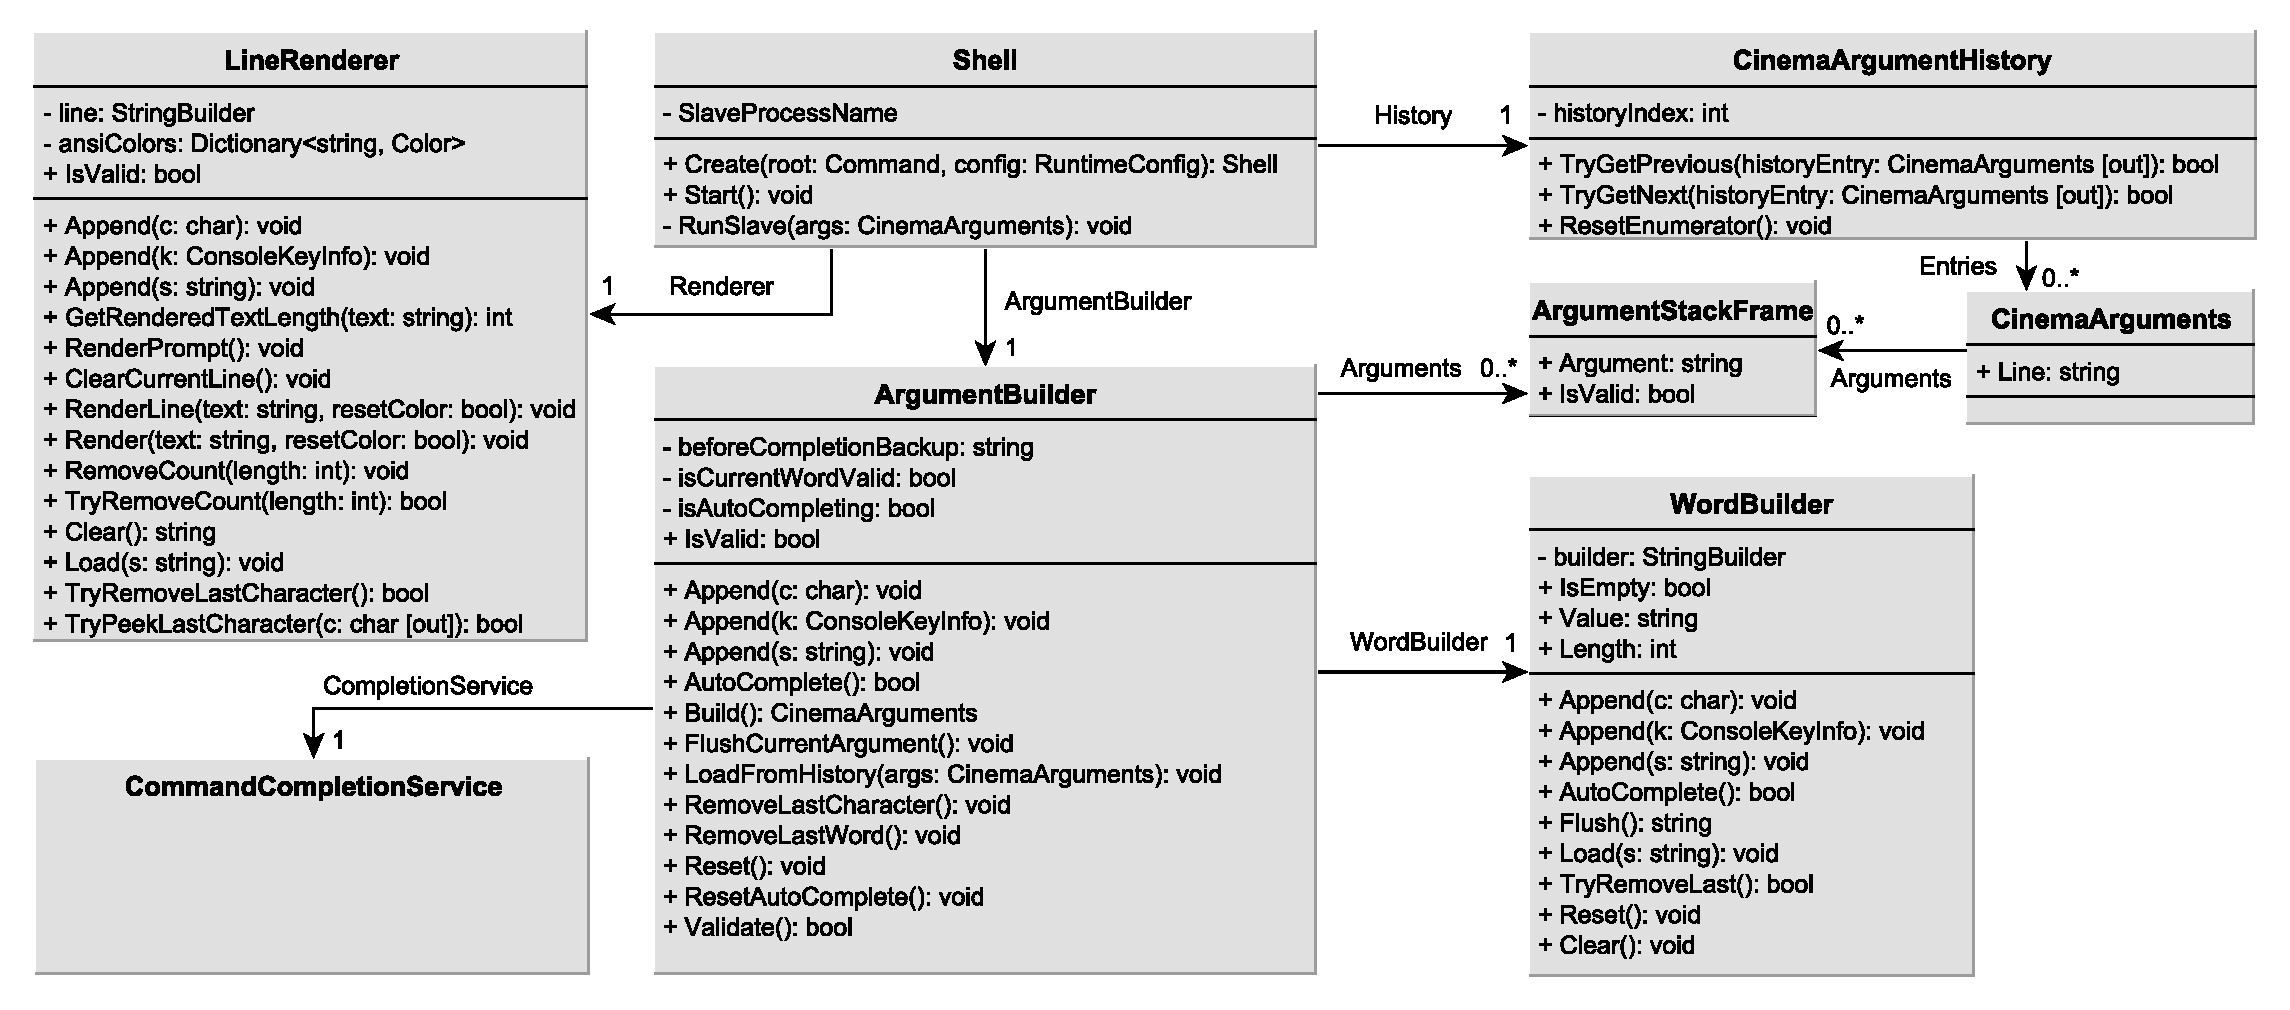
\includegraphics[width=\textwidth]{images/client-wrapper}
    \caption{Architecture of the client wrapper application.}
    \label{fig:client-wrapper}
\end{figure}

As shown in Figure \ref{fig:client-wrapper}, the core class of the wrapper is the \inlinecode{Shell} class, which is responsible for monitoring key presses, managing dependent classes, and slaving the client application to the current command line.

When the \inlinecode{Shell::Start()} method is invoked, a prompt is rendered to the screen using the \inlinecode{LineRenderer} class, which also offers support for parsing \gls{a:ansi} color codes. As soon as a key press event is raised, the following parsing algorithm is executed:

\begin{enumerate}
    \item The key information is read, and depending on the character, one of these actions is taken:
    \begin {enumerate}
        \item For alphanumeric \gls{a:ascii} characters or symbols, the character is appended to the \inlinecode{ArgumentBuilder} and \inlinecode{LineRenderer}. The \inlinecode{ArgumentBuilder} updates its internal \inlinecode{WordBuilder} instance accordingly.
        \item For arrow keys (up or down), the previous or next command from the command history is retrieved using the \inlinecode{CinemaArgumentsHistory} class. The \inlinecode{ArgumentBuilder} and \inlinecode{LineRenderer} are updated, the prompt is redrawn, and the key parsing process \textbf{concludes} and is ready to handle the next key press.
        \item For a backspace key, the last character or word (depending on whether the control key is also pressed) is removed from the \inlinecode{ArgumentBuilder} and \inlinecode{LineRenderer}. The \inlinecode{ArgumentBuilder} updates its internal \inlinecode{WordBuilder} instance accordingly.
        \item For a space or enter key, the \inlinecode{ArgumentBuilder} flushes it's current word, validates the new argument against the syntax tree by invoking the \inlinecode{CommandCompletionService}, and pushes the argument onto the argument stack.
        \begin{enumerate}
            \item If the enter key is pressed, the renderer completes the current line, the \inlinecode{ArgumentBuilder} is flushed, and a new line is rendered. The client application is then spawned as a slave process, forwarding input, output, and error streams to the master. When the client process exits, the key parsing \textbf{concludes} and is ready to handle the next key press.
            \item Otherwise, if the key is a space, the space character is added to the renderer.
        \end{enumerate}
        \item Any other keys are ignored for now.
    \end{enumerate}
    \item The \inlinecode{ArgumentBuilder} validates its current argument stack and partial argument against the syntax tree.
    \begin{enumerate}
        \item If the argument is valid, it is passed to the \inlinecode{CommandCompletionService}, and the autocomplete cache is updated accordingly. The \inlinecode{CommandCompletionService} returns a list of possible completions for the current argument.
        \item Otherwise, the renderer is updated to re-render the current line in red for the next call to \inlinecode{RenderPrompt()}.
    \end{enumerate}
    \item One of the following actions is taken:
    \begin{enumerate}
        \item If the key is a tab key, the current partial input is backed up, and one of these actions is taken:
        \begin{enumerate}
            \item If the autocomplete cache is empty, the cache is updated by invoking the \inlinecode{CommandCompletionService} with the current argument.
            \item Otherwise, the autocomplete cache is queried for possible completions for the current argument.
            \begin{enumerate}
                \item If the previous key was also a tab key, the next completion in the autocomplete cache is returned.
                \item Otherwise, the first completion in the autocomplete cache is returned.
                \item If the autocomplete cache is empty or no next completion exists, the backup is restored.
            \end{enumerate}
            \item The \inlinecode{ArgumentBuilder} and \inlinecode{LineRenderer} are updated with the new completion.
        \end{enumerate}
        \item Otherwise, the autocomplete cache is reset.
    \end{enumerate}
    \item The current line is re-rendered.
    \item The key parsing concludes and is ready to handle the next key press.
\end{enumerate}

Overall, the shell wrapper aims to provide seamless integration of the client application into the shell environment, enabling a more intuitive user experience.
